\PassOptionsToPackage{numbers,compress}{natbib}
\documentclass{article}
% ES 678 course paper. Uses the official NeurIPS 2025 style; replace with the
% course starter's style file (same interface) before final submission if required.
\usepackage[preprint]{neurips_2025}

\usepackage[utf8]{inputenc}
\usepackage[T1]{fontenc}
\usepackage{hyperref}
\usepackage{url}
\usepackage{booktabs}
\usepackage{amsfonts,amsmath,amssymb,amsthm}
\usepackage{nicefrac}
\usepackage{microtype}
\usepackage{graphicx}
\usepackage{xcolor}

\newtheorem{observation}{Observation}
\newcommand{\Df}{\mathcal{D}_f}
\newcommand{\Dr}{\mathcal{D}_r}
\newcommand{\D}{\mathcal{D}}

\title{Forgetting the Pipeline Too: Fast Tabular Machine Unlearning under Preprocessing and Imputation Shifts}

\author{%
  Ojas Gupta \\
  Roll No.\ 26250031 \quad ES 678: Machine Learning\\
  Indian Institute of Technology Gandhinagar\\
  \texttt{ojasgupta@iitgn.ac.in} \\
}

\begin{document}
\maketitle

\begin{abstract}
Machine unlearning methods update model weights after a deletion request but usually treat the
feature map as fixed. In tabular pipelines the feature map is itself learned: imputation means,
scaling statistics and target encodings are fitted on the training set and keep a trace of
deleted records. We study this on 30-day readmission prediction with 25{,}000 encounters from the
UCI Diabetes 130-US Hospitals data, deleting the most heavily utilizing patients. Freezing the
preprocessor leaves the deleted cohort in the deployed statistics (e.g.\ the scale of
\texttt{number\_inpatient} stays at 1.20 instead of 0.78), and a standard influence (Newton) update
then lands \emph{further} from the retrained weights than doing nothing (5/5 seeds), even though it
does improve predictions. We propose PLU-GGN, which downdates the preprocessor exactly from the
deleted rows' sufficient statistics and adds a pipeline-shift term to the Gauss--Newton step. At 3\%
deletion it cuts weight error 26$\times$ relative to standard influence (one step) and to
$2.4\times10^{-5}$ with a second step, at about 5$\times$ the speed of retraining. We also show
that a feature-norm membership audit we first used reports 0.95--0.999 AUC only because the
deleted patients are extreme; against equally extreme held-out patients it falls to about 0.53--0.56.
\end{abstract}

\section{Problem, data and scope}
\label{sec:problem}
Data-protection laws (India's DPDP Act 2023, GDPR Art.~17) let patients withdraw consent. A
hospital model should then behave as if those patients had never been used. The reference answer
is \emph{oracle retraining}: refit the whole pipeline on the retained data. The question here is
\textbf{how closely cheap unlearning updates match oracle retraining when the preprocessing is
also learned from the data, and what a frozen preprocessor leaks.} The question is about unlearning
fidelity, not about building the best readmission model.

\textbf{Task and unit.} One row is one inpatient encounter of a diabetic patient (UCI Diabetes
130-US Hospitals, 1999--2008~\cite{strack2014}, CC BY 4.0, via OpenML id 4541; we use a fixed random
sample of 25{,}000 of 101{,}766 encounters). The target is readmission within 30 days (11.2\%
positive). The prediction is made at discharge, so we use only information available then: 8 counts
(\texttt{time\_in\_hospital}, \texttt{num\_lab\_procedures}, \texttt{num\_procedures},
\texttt{num\_medications}, prior-year \texttt{number\_outpatient/emergency/inpatient},
\texttt{number\_diagnoses}) and 4 categoricals (admission type, discharge disposition, medical
specialty, A1C result).

\textbf{Data quality.} The counts are heavily right-skewed (\texttt{number\_emergency}: median 0,
99th percentile 4, max 76). \texttt{medical\_specialty} is missing for 49\% of encounters and is kept
as its own level. The released numeric columns have no missing values, so to exercise the imputer
we mask 12\% of numeric cells \emph{completely at random}; this is a simulation, and real clinical
missingness is rarely MCAR. The 25{,}000 encounters come from 22{,}171 patients, so we split by
patient (\texttt{GroupShuffleSplit}, seed 42): 19{,}995 training and 5{,}005 test encounters, with
zero shared patients. All preprocessing is fitted on training rows only.

\textbf{Deletion request.} The forget cohort $\Df$ is the top $q\%$ of training encounters by
utilization $3\cdot\texttt{number\_inpatient}+0.1\cdot\texttt{num\_lab\_procedures}$ (default $q=3$,
$|\Df|=599$). This is a deliberately hard case: high-leverage patients move the pipeline the most.
We repeat everything with uniformly random cohorts as a control.

\section{Method}
\label{sec:method}
Let $\phi_\D$ be the preprocessor fitted on $\D$ and
$L(\theta;\D,\phi)=\sum_{i\in\D}\ell(\theta^\top\phi(x_i),y_i)+\tfrac12\theta^\top\Lambda\theta$
be the L2-regularized logistic loss ($\Lambda=\mathrm{diag}(10,\dots,10,10^{-4})$, intercept last).
The oracle is $\theta_r^*=\arg\min_\theta L(\theta;\Dr,\phi_{\Dr})$ with $\Dr=\D\setminus\Df$.
$\phi$ does mean imputation, standardization, and Empirical-Bayes target encoding
$(\sum_{c}y+m\bar y)/(n_c+m)$ with $m=10$. $\lambda$ and $m$ were fixed in advance; nothing is
tuned on the test set.

\textbf{Baselines.} (i) \emph{No unlearning} ($\hat\theta$, $\phi_\D$). (ii) \emph{Gradient ascent}:
5 steps of size $10^{-4}$ on the $\Df$ loss. (iii) \emph{Standard influence / GGN removal}~\cite{koh2017,guo2020}:
$\theta_{\mathrm{SI}}=\hat\theta+G(\hat\theta;\Dr,\phi_\D)^{-1}g_{\mathrm{rem}}$ with
$g_{\mathrm{rem}}=\sum_{i\in\Df}\nabla_\theta\ell(\hat\theta^\top\phi_\D(x_i),y_i)$. (ii) and (iii) keep $\phi_\D$ frozen.

\begin{observation}[Two parts of the shift]
$\theta_r^*-\hat\theta=\underbrace{[\theta^*(\phi_\D,\Dr)-\hat\theta]}_{\text{sample removal}}+
\underbrace{[\theta^*(\phi_{\Dr},\Dr)-\theta^*(\phi_\D,\Dr)]}_{\text{coordinate change}}$.
Standard influence approximates only the first term. When $\Df$ holds high values of feature $j$,
removing it shrinks $\sigma_j$, so a fixed effect per raw unit needs a \emph{smaller} coefficient per
standardized unit, while removing the cohort's own gradient pushes the same coefficient the other
way. If the two parts point in opposite directions, $\theta_{\mathrm{SI}}$ can be further from
$\theta_r^*$ than $\hat\theta$ is.
\end{observation}
This is an identity plus an argument about direction, not a theorem; Section~\ref{sec:results}
checks it empirically.

\textbf{PLU-GGN.} \emph{Step 1, exact preprocessor downdate.} We store additive statistics
$(n^{\mathrm{obs}}_j,\sum x_{ij},\sum x_{ij}^2)$ per numeric column and $(n_c,\sum_{c}y)$ per
category level, subtract those of $\Df$, and recompute $\phi_{\Dr}$ in $O(|\Df|)$. The stored retain
matrix is then re-expressed by the affine map $z^{\mathrm{new}}=(\sigma^{\mathrm{old}}_j/\sigma^{\mathrm{new}}_j)z^{\mathrm{old}}
+(\mu^{\mathrm{old}}_j-\mu^{\mathrm{new}}_j)/\sigma^{\mathrm{new}}_j$ (imputed cells stay 0; categorical
columns are re-mapped). \emph{Step 2, coupled gradient.} Expanding the optimality condition of
$\theta_r^*$ around $(\hat\theta,\phi_\D)$ gives the extra term
$g_{\mathrm{shift}}=\sum_{i\in\Dr}[\nabla_\theta\ell(\hat\theta^\top\phi_{\Dr}(x_i),y_i)-\nabla_\theta\ell(\hat\theta^\top\phi_\D(x_i),y_i)]$.
\emph{Step 3, GGN step} in the new coordinates:
$\theta_{\mathrm{PLU}}=\hat\theta+G_{\mathrm{new}}^{-1}(g_{\mathrm{rem}}-g_{\mathrm{shift}})$ with
$G_{\mathrm{new}}=X_{r,\mathrm{new}}^\top\mathrm{diag}(p_i(1-p_i))X_{r,\mathrm{new}}+\Lambda$.
PLU-GGN-2 adds one further (undamped) Newton step on $L(\cdot;\Dr,\phi_{\Dr})$.
\textbf{Cost.} Only Step 1 is $O(|\Df|)$. Steps 2--3 make one pass over $\Dr$ ($O(|\Dr|d^2+d^3)$, $d=13$)
but need no iterative optimization. So PLU-GGN is cheaper than retraining, not independent of $|\Dr|$.

\section{Evaluation design}
\label{sec:eval}
The split, the forget-cohort rule, $\lambda$ and $m$ were fixed before comparing methods. Every method
is compared with the oracle for the same request. \textbf{Weight error} $\|\theta-\theta_r^*\|_2$ is
the usual unlearning metric, but frozen-$\phi$ methods express $\theta$ in different coordinates, so
we also report a frame-free \textbf{function-space error}: mean Bernoulli KL between oracle and method
predictions on the held-out test set. \textbf{Pipeline leak} is
$\sum_j(|\Delta\mu_j|+|\Delta\sigma_j|)$ relative to the oracle preprocessor, normalized so that the
frozen $\phi_\D$ scores 100\%. We report test PR-AUC (appropriate at 11\% prevalence) only to check
that unlearning does not damage the model; the prevalence baseline is 0.112 and a one-feature
\texttt{number\_inpatient} score reaches 0.168. Timings are medians of 7 runs on one CPU core
(NumPy/SciPy, x86-64). Because L-BFGS alone stops $\sim\!10^{-5}$ from the optimum, the oracle
reference is polished with three Newton steps (gradient norm $\sim\!10^{-13}$); only the L-BFGS refit is timed. We repeat the 3\% experiment over 5 seeds that change both the patient split
and the missingness mask.

\section{Results}
\label{sec:results}
\begin{table}[t]
\caption{Deleting the 3\% highest-utilization training encounters ($|\Df|=599$, $|\Dr|=19{,}396$,
$|\D_{\mathrm{test}}|=5{,}005$, seed 42). KL and max\,$|\Delta p|$ are against oracle predictions on
the test set. Last column: mean $\pm$ s.d.\ of weight error over 5 split/mask seeds.}
\label{tab:main}
\centering\footnotesize
\setlength{\tabcolsep}{2.6pt}
\begin{tabular}{lcccccc}
\toprule
Method & Weight err.\,$\downarrow$ & Test KL\,$\downarrow$ & max\,$|\Delta p|$ & Pipe leak & Speedup & Weight err.\ (5 seeds)\\
\midrule
Oracle retrain & 0 & 0 & 0 & 0\% & 1$\times$ (90\,ms) & 0\\
No unlearning & $1.25\times10^{-1}$ & $3.7\times10^{-4}$ & 0.118 & 100\% & -- & $0.123\pm0.018$\\
Grad.\ ascent, frozen $\phi$ & $1.71\times10^{-1}$ & $1.2\times10^{-4}$ & 0.060 & 100\% & $\sim\!10^3\times$ & $0.173\pm0.017$\\
Std.\ influence, frozen $\phi$ & $1.55\times10^{-1}$ & $7.7\times10^{-5}$ & 0.062 & 100\% & 63$\times$ & $0.151\pm0.008$\\
PLU-GGN 1-step & $5.98\times10^{-3}$ & $4.4\times10^{-6}$ & 0.013 & 0\% & 5.5$\times$ & $(4.7\pm0.9)\times10^{-3}$\\
PLU-GGN 2-step & $2.42\times10^{-5}$ & $7.3\times10^{-11}$ & $5\times10^{-5}$ & 0\% & 5.1$\times$ & $(1.4\pm0.6)\times10^{-5}$\\
\bottomrule
\end{tabular}
\end{table}

\begin{figure}[t]
\centering
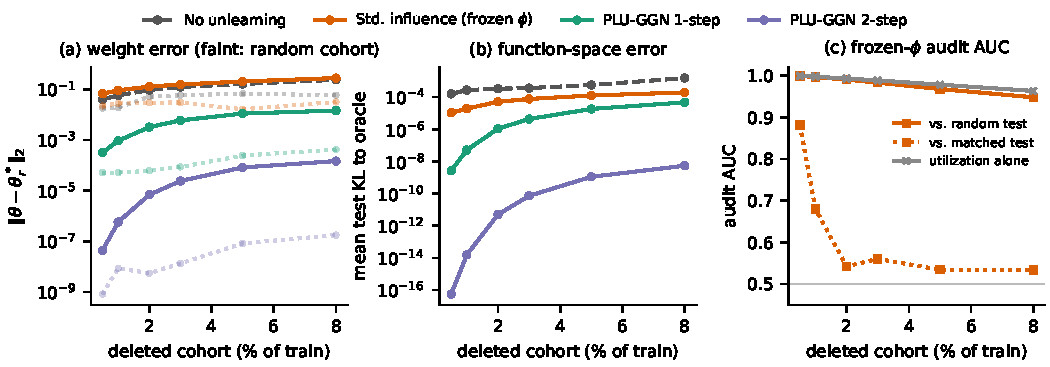
\includegraphics[width=\linewidth]{figures/fig_ablation.pdf}
\caption{Deletion-fraction sweep (top-utilization cohorts). (a) Weight error; faint dotted lines are
random cohorts of the same size. (b) Function-space error on the test set. (c) The feature-norm
membership audit for the frozen preprocessor, scored against random test patients versus
utilization-matched test patients, and the AUC of the utilization score alone.}
\label{fig:ablation}
\end{figure}

\textbf{Main comparison (Table~\ref{tab:main}).} The frozen preprocessor keeps the deleted cohort:
the standardization scale of \texttt{number\_inpatient} is 1.20 under $\phi_\D$ and 0.78 under
$\phi_{\Dr}$. As the Observation predicts, standard influence ends further from $\theta_r^*$ than no
unlearning (0.155 vs.\ 0.125; this held on all 5 seeds). The largest single discrepancy is the
\texttt{number\_inpatient} coefficient: oracle 0.253, full model 0.328, standard influence 0.390,
so the removal step moves it the wrong way. In \emph{function space}, however, standard influence
is still 4.8$\times$ closer to the oracle than doing nothing. Its failure is mostly in parameters,
which matters for certified-removal guarantees stated on $\theta$~\cite{guo2020}. PLU-GGN with one
step reduces weight error 26$\times$ relative to standard influence; the second step reaches
$2.4\times10^{-5}$. All methods have test PR-AUC within 0.208--0.210, well inside the
$\pm0.020$ seed-to-seed spread, so unlearning does not change predictive quality; the model itself is
modest (ROC-AUC 0.66, PR-AUC 0.21 vs.\ 0.11 prevalence). Retraining takes only 90\,ms here, so the
$\approx$5$\times$ speedup (4.5--5.7$\times$ across sizes and seeds) matters for larger pipelines, not for this one.

\textbf{Sensitivity to deletion size and cohort type (Fig.~\ref{fig:ablation}a,b).} One-step error
grows with the deletion fraction ($3.2\times10^{-4}$ at 0.5\% to $1.5\times10^{-2}$ at 8\%) because
the Taylor expansion is less accurate for large shifts; the second step brings it to
$4\times10^{-8}$--$1.5\times10^{-4}$. For \emph{random} cohorts the pipeline barely moves: standard influence is
worse than doing nothing only at 0.5--1\% deletion, and PLU-GGN-1 already reaches $\le4.3\times10^{-4}$.
So the coordinate-shift failure is specific to high-leverage deletions, which are exactly the
patients most likely to be identifiable.

\textbf{Failure audit: what the membership test measures (Fig.~\ref{fig:ablation}c).} Our first
privacy test scored each record by $\|\phi_{\Dr}(x)\|-\|\phi_{\mathrm{deployed}}(x)\|$ and reported
0.95--0.999 AUC for deleted vs.\ random test patients under a frozen $\phi_\D$, and exactly 0.5 for
PLU-GGN. Both numbers are misleading. The score depends only on $x$, not on whether $x$ was in
training, so it cannot separate a member from a non-member with the same features; and it is
identically zero whenever $\phi_{\mathrm{deployed}}=\phi_{\Dr}$, so PLU-GGN's 0.5 holds by
construction. Its high AUC comes from comparing extreme deleted patients with ordinary test patients:
the raw utilization score alone gets 0.96--0.999. Against held-out patients at least as extreme as the
least extreme deleted one, the audit falls to 0.53--0.56 for deletions of $\ge2\%$ (0.68--0.88 for
0.5--1\%, where only 30--41 matched controls exist). For random cohorts it is 0.51--0.55. The leakage
that \emph{is} real is aggregate: a frozen $\phi_\D$ deploys statistics that include $\Df$, and if both
$\phi_\D$ and a retrained $\phi_{\Dr}$ are ever exposed, differencing their sufficient statistics recovers
the deleted cohort's mean \texttt{number\_inpatient} exactly (5.37 vs.\ 0.47 for retained patients),
a classic differencing attack~\cite{dinur2003}. PLU-GGN removes the first problem (pipe leak 0\%) but
not the second; that would need noise, as in certified removal~\cite{guo2020}.

\textbf{Representative errors.} PLU-GGN-1's largest test-prediction errors are on the most extreme
held-out patients (top 0.2\% utilization, 8--9 prior inpatient visits), where $|\Delta p|\approx0.012$
around oracle risks of 0.43--0.58; the median $|\Delta p|$ is $1.1\times10^{-4}$, and $|\Delta p|$ has
rank correlation 0.56 with utilization. Residual error therefore sits where the curvature
approximation is worst, which is another reason to take the second step.

\section{Limitations and conclusion}
\label{sec:limits}
(1) Exact $O(|\Df|)$ downdates exist only for additive statistics; median or $k$-NN imputation and
quantile scaling need sketches or approximate updates. (2) Missingness is simulated MCAR. (3) We study
one convex model with $d=13$; for non-convex models the GGN step is only local. (4) The single fixed
utilization rule defines the hard case; other request patterns (e.g.\ all encounters of one patient)
are untested. (5) The membership audit is weak by design (above), so we make no per-patient privacy
claim. (6) The readmission associations come from observational data and are not causal effects.
\textbf{Conclusion.} When preprocessing is learned, unlearning must update it too. Doing so exactly is
cheap for additive statistics, and adding the pipeline-shift gradient brings a one- or two-step update
to within $10^{-2}$--$10^{-5}$ of retraining. Without it, standard influence can move weights the
wrong way on exactly the high-leverage deletions where it matters most.

\textbf{Reproducibility and AI use.} Code, the cached data sample, all results and an in-browser
replication are at \url{https://github.com/Ojas1024/plu-ggn-unlearning};
\texttt{python experiments/run\_all.py} regenerates every number here in under a minute. AI assistants
(Claude, Anthropic) were used for code refactoring, re-running and auditing experiments (including
the matched-control audit), building the website and editing text; the author checked all reported results.

{\small
\begin{thebibliography}{9}\setlength{\itemsep}{0pt}
\bibitem{strack2014} B.~Strack et al. Impact of HbA1c measurement on hospital readmission rates: analysis of 70{,}000 clinical database patient records. \emph{BioMed Research International}, 2014.
\bibitem{koh2017} P.~W. Koh and P.~Liang. Understanding black-box predictions via influence functions. In \emph{ICML}, 2017.
\bibitem{guo2020} C.~Guo, T.~Goldstein, A.~Hannun, and L.~van~der~Maaten. Certified data removal from machine learning models. In \emph{ICML}, 2020.
\bibitem{dinur2003} I.~Dinur and K.~Nissim. Revealing information while preserving privacy. In \emph{PODS}, 2003.
\end{thebibliography}
}
\end{document}
